\documentclass[a4paper, 11pt]{article}
\usepackage[polish]{babel}
\usepackage[MeX]{polski}
\usepackage[utf8]{inputenc}
\usepackage[T1]{fontenc}
%\usepackage{times}
\usepackage{graphicx,wrapfig}
%\usepackage{anysize}
%\usepackage{tikz}
%\usetikzlibrary{calc,through,backgrounds,positioning}
\usepackage{anysize}
\usepackage{float}
%\usepackage{stmaryrd}
%\usepackage{amssymb}
%\usepackage{amsthm}
%\marginsize{3cm}{3cm}{3cm}{3cm}
%\usepackage{amsmath}
%\usepackage{color}
%\usepackage{listings}
%\usepackage{enumerate}
%\lstloadlanguages{Ada,C++}

\usepackage{listings} %do impotu kodu
\author{Marcin Jędrzejczyk \and Sebastian Katszer }
\title{Projekt UML Automatu z przekąskami }


\newcommand{\HRule}{\rule{\linewidth}{0.5mm}} % Defines a new command for the horizontal lines, change thickness here
\newtheorem{defi}{Definicja}
\renewcommand{\contentsname}{Spis treści}
\renewcommand{\refname}{Bibliografia}
\renewcommand{\figurename}{Rysunek}


\begin{document}

%\maketitle	%robi stronê tytu³ow±
\begin{titlepage}


\center % Center everything on the page
%----------------------------------------------------------------------------------------
%	HEADING SECTIONS
%----------------------------------------------------------------------------------------

\textsc{\LARGE Akademia Górniczo-Hutnicza    \\im. Stanisława Staszica w Krakowie}\\[1.5cm] % Name of your university/college
\textsc{\Large Analiza i modelowanie oprogramowania}\\[0.5cm] % Major heading such as course name
%\textsc{\large Minor Heading}\\[0.5cm] % Minor heading such as course title

%----------------------------------------------------------------------------------------
%	TITLE SECTION
%----------------------------------------------------------------------------------------

\HRule \\[0.4cm]
{ \huge \bfseries Projekt UML Automatu z przekąskami}\\[0.4cm] % Title of your document
\HRule \\[5.5cm]
 
%----------------------------------------------------------------------------------------
%	AUTHOR SECTION
%----------------------------------------------------------------------------------------

\begin{minipage}{0.4\textwidth}
\begin{flushleft} \large 
\emph{Autorzy:}\\
Marcin \textsc{Jędrzejczyk} \\
Sebastian \textsc{Katszer}\\

\end{flushleft}
\end{minipage}
~
\begin{minipage}{0.4\textwidth}
\begin{flushright} \large
\emph{Prowadzący:}\\
 Dr inż. Wojciech \textsc{Szmuc} % Supervisor's Name
\end{flushright}
\end{minipage} \\[5cm]

{\large \today}\\[3cm]
\vfill
\end{titlepage}
%----------------------------------------------------------------------------------------
%	DOCUMENT SECTION
%----------------------------------------------------------------------------------------
%\tableofcontents %robi spis tre¶ci	- 3 kompilacje
\newpage
\section{Automat z przekąskami }
\subsection{Co to jest?}
 Automat sprzedający (automat vendingowy, ang. vending machine) – urządzenie służące do sprzedaży samoobsługowej. Można wyróżnić automaty sprzedające towary i usługi.\\
 Największymi producentami automatów vendingowych na świecie są Chiny, USA, Włochy i Hiszpania.
 Polskie przedsiębiorstwa prowadzące działalność wendingową skupia Polskie Stowarzyszenie Vendingu.
\subsection{Analiza wymagań}
\emph{Analiza wymagań}– uzgodnienie wymagań klienta i ich analiza. Celem jest określenie zakresu prac, oszacowanie czasochłonności, kosztów i czasu wykonania.\\[1cm] 
\begin{tabular}{|l|p{3.5cm}|l|l|l|} \hline
ID  & OPIS & PRIORYTET & KRYTYCZNOŚĆ & HARMONOGRAM \\ \hline
R01 & Wydawanie reszty & Wysoki & Średnia & Release 1\\ \hline
R02 & Dostęp techniczny dla osób upoważnionych & Wysoki & Wysoka & Release 1 \\ \hline
R03 & Sposób inicjalizacji & Średni & Średnia & Release 1\\ \hline
R04 & Wydawanie produktu & Średni & Średnia & Release 1 \\ \hline
\end{tabular}\\


\newpage
\section{Diagram przypadków użycia}
\emph{Diagram przypadków użycia}– graficzne przedstawienie przypadków użycia, aktorów oraz związków między nimi, występujących w danej dziedzinie przedmiotowej.
\begin{figure}[ht]
\centerline{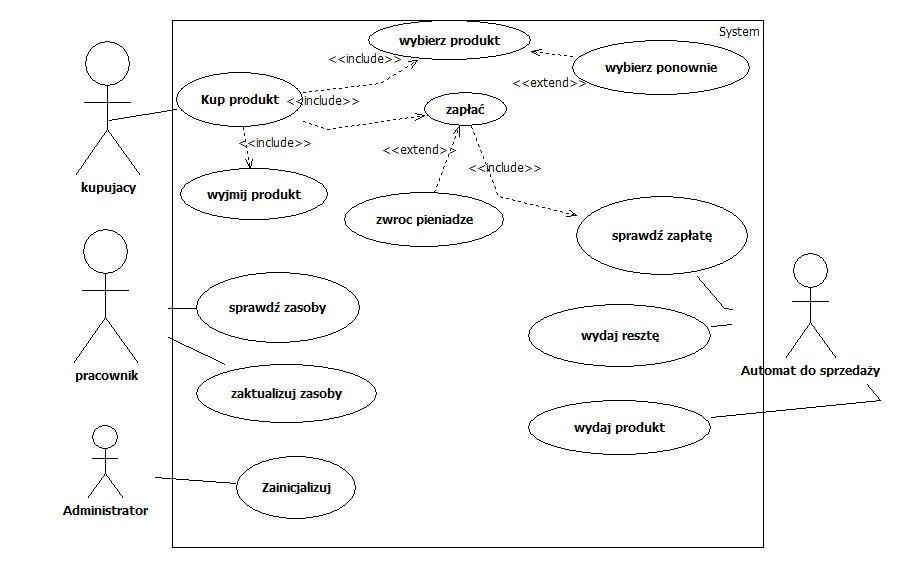
\includegraphics[scale=0.6]{uzycia}}
\caption{Diagram przypadków użycia}
\end{figure}%

\newpage
\subsection{Diagram sekwencji}
\emph{Diagramy sekwencji} - opisują interakcje pomiędzy częściami systemu w postaci sekwencji komunikatów wymienianych między nimi.\\[1cm] 
\begin{figure}[ht]
\centerline{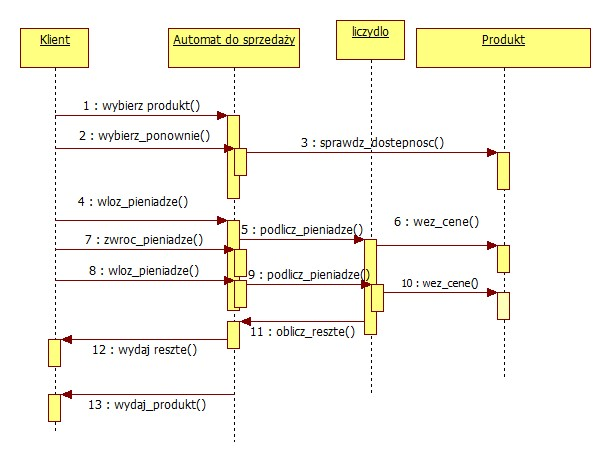
\includegraphics[scale=0.8]{sekwencje}}
\caption{Diagram sekwencji}
\end{figure}

%\bibliographystyle{unsrt}
%\bibliography{bib2}
\end{document}
